% DO LE DUY
% 1026-32-2038
% July 7 2020

\documentclass[11pt]{article}
\usepackage{graphicx}
\graphicspath{ {./graphic/} }
\usepackage[T1]{fontenc}
\usepackage[bitstream-charter]{mathdesign}
\title{Practice of Basic Informatics - Homework 8}
\usepackage{float}
\usepackage{geometry}
\geometry{left=2cm,right=2cm,top=1cm,bottom=2cm,includeheadfoot}
\author{by Do Le Duy}
\date{\today}

\begin{document}

\maketitle
\section{Graphic 1}

\begin{figure}[H] 
    \begin{center} 
        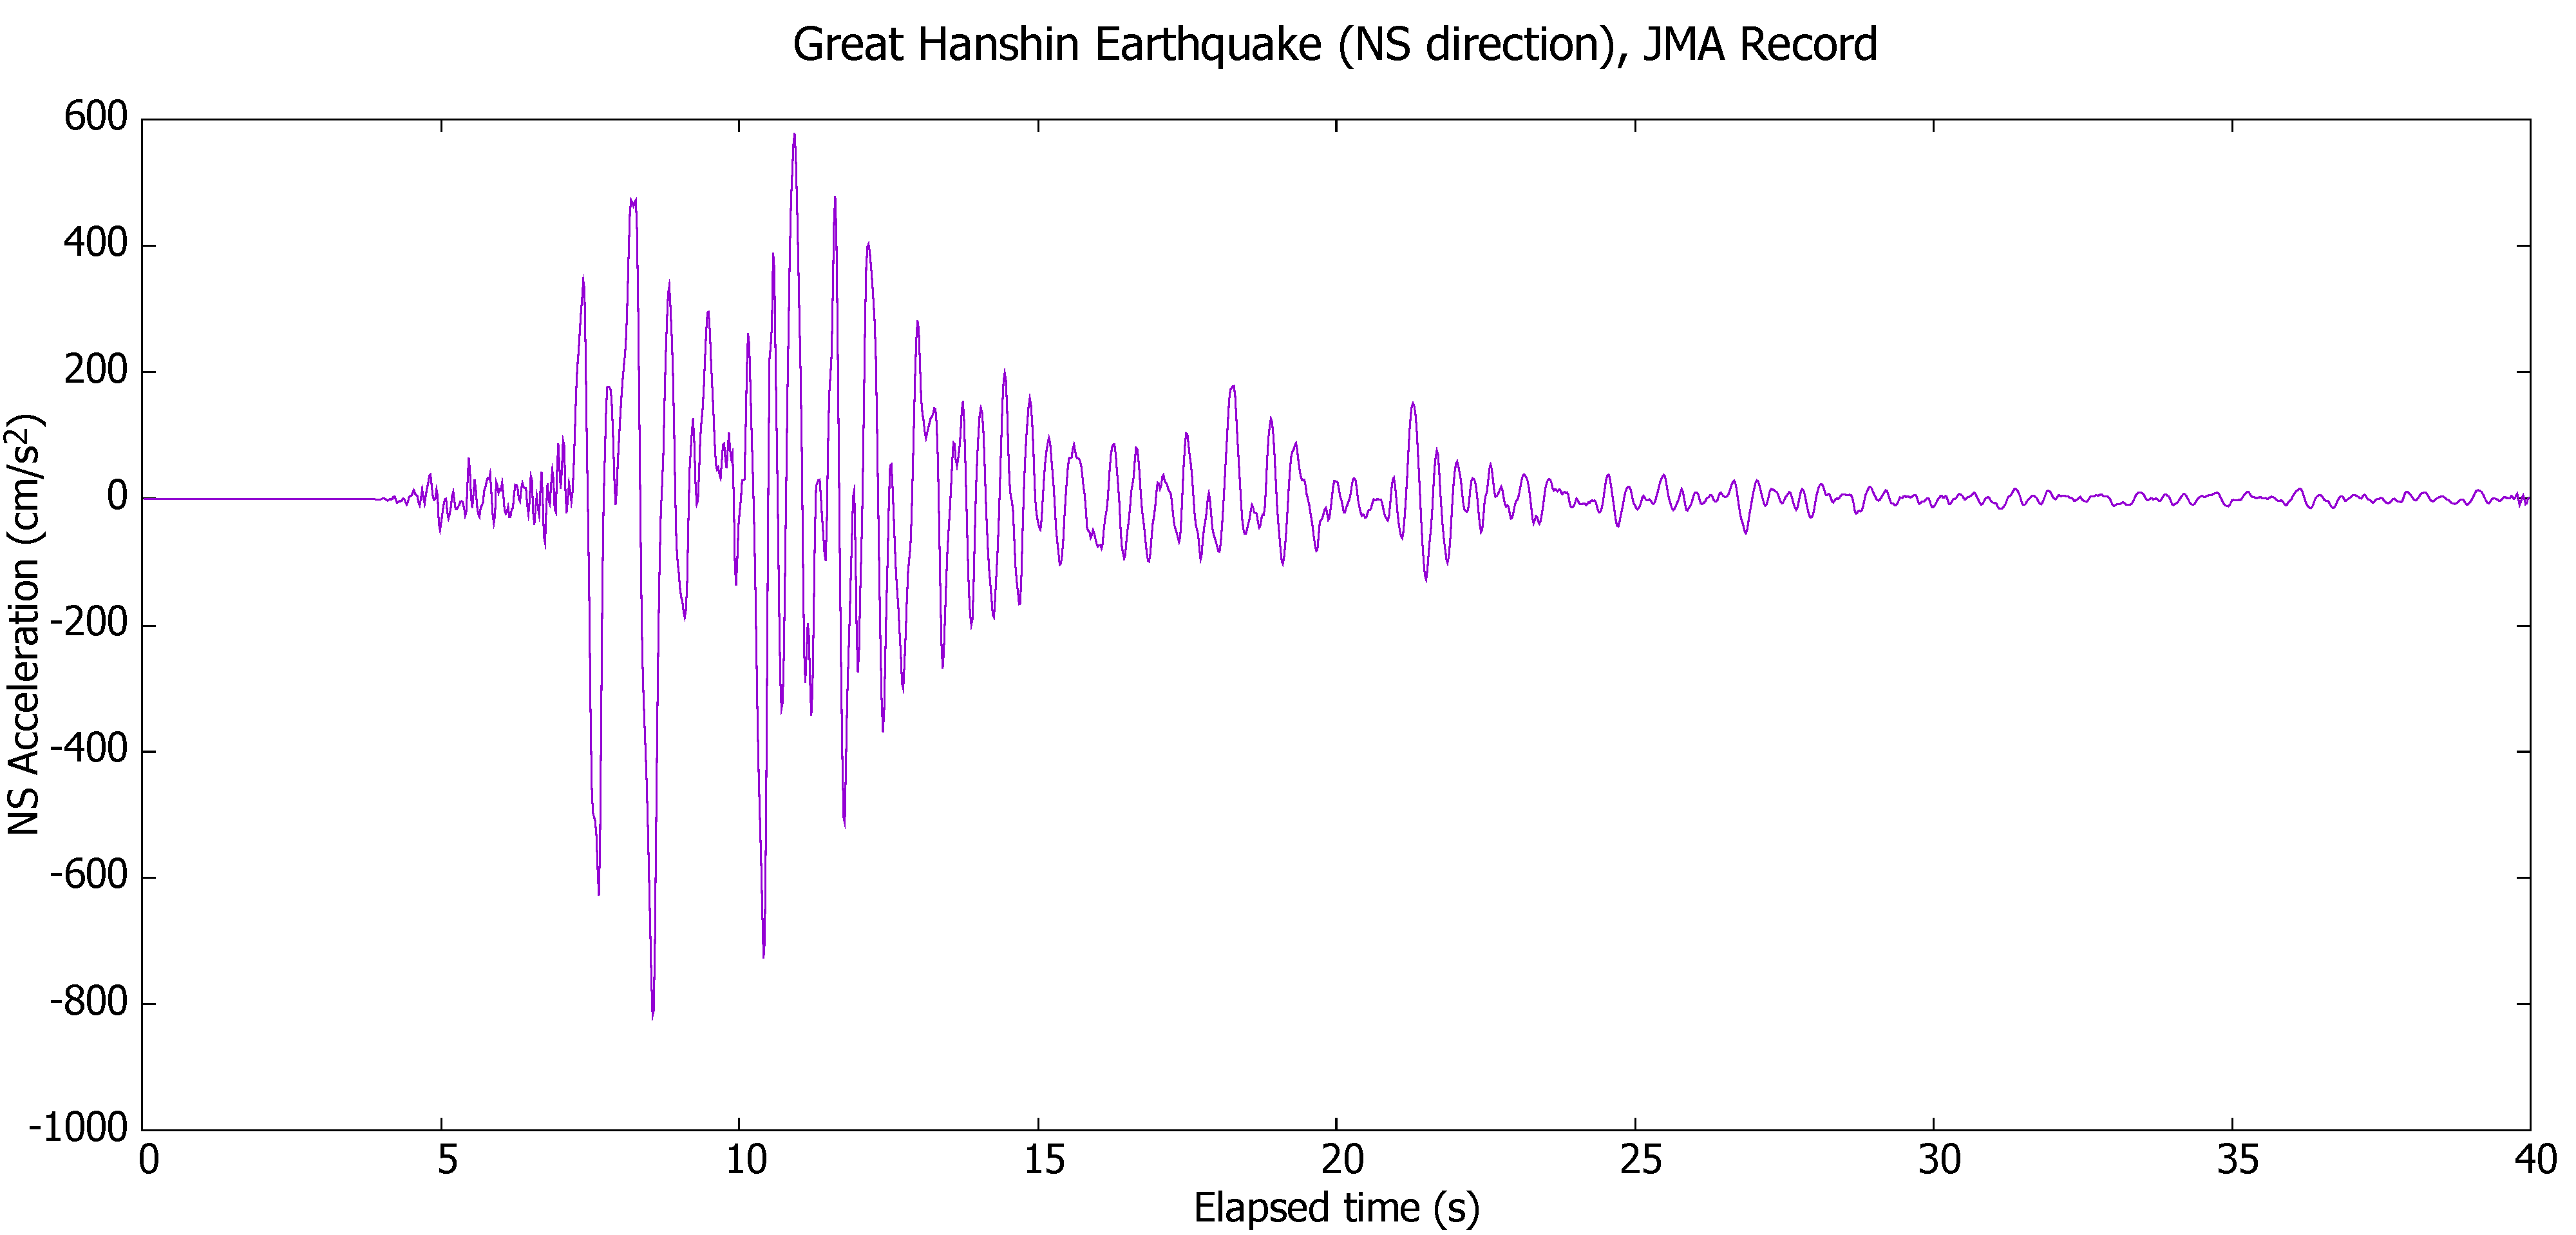
\includegraphics[scale=0.25]{1} 
    \end{center} 
    \caption{North-south seismic wave (recorded acceleration) observed in the
    Kobe Marine Observatory, due to the Hyogo Prefecture earthquake of 1995.} 
\end{figure}

\section{Graphic 2}
\begin{figure}[H] 
    \begin{center} 
        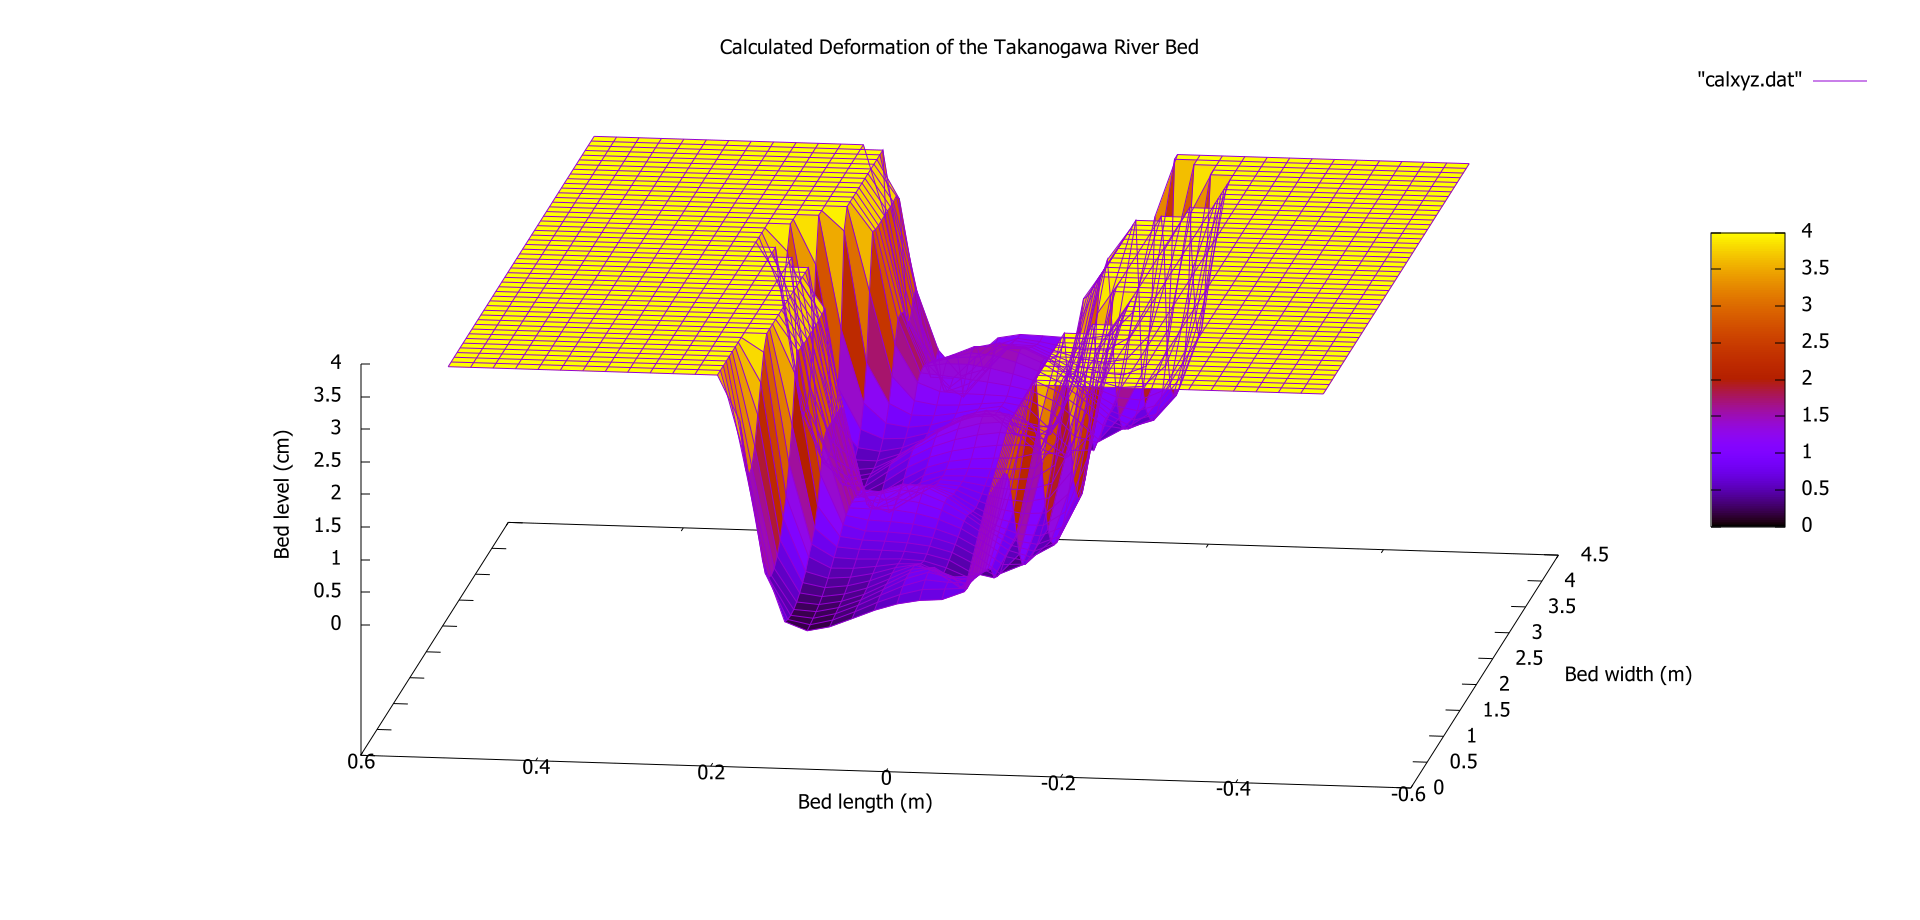
\includegraphics[scale=0.25]{2} 
    \end{center} 
    \caption{A numerical simulation of the development of river sandbars and meanders} 
\end{figure}

\section{Graphic 3}
\begin{figure}[H] 
    \begin{center} 
        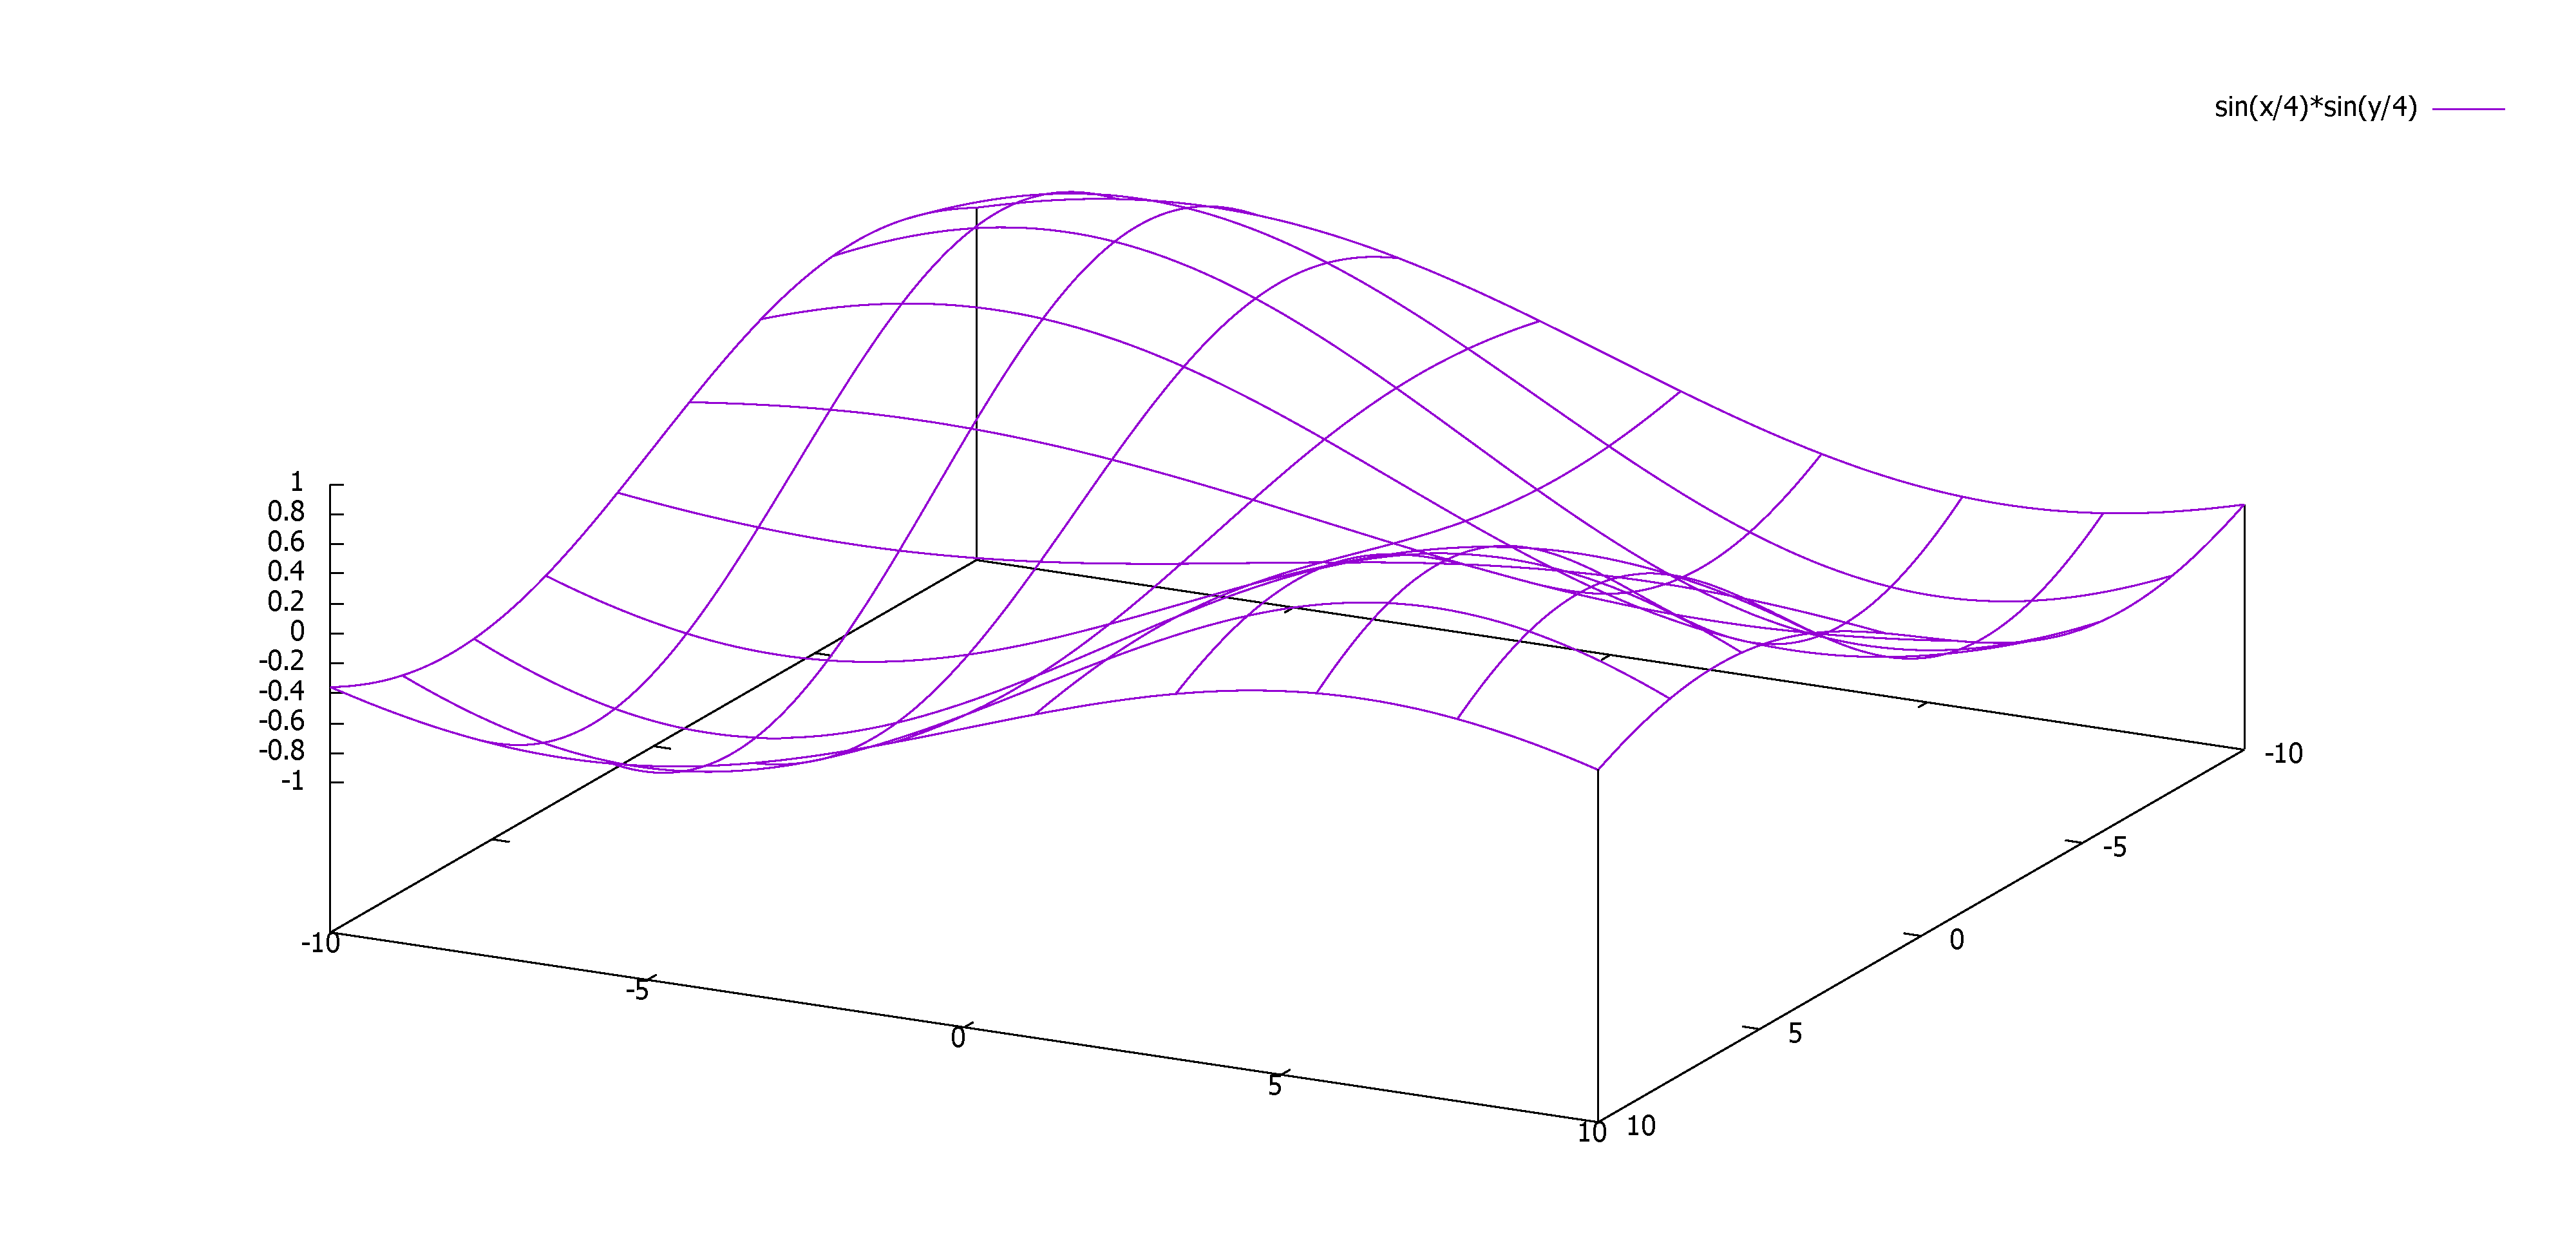
\includegraphics[scale=0.25]{3} 
    \end{center} 
    \caption{A 2D Standing Wave Patterns} 
\end{figure}
The general form of standing wave in two dimensions is: 
\[\psi(x, y)_{n_{x}, n_{y}}=A_{n_{x}, n_{y}} \sin \left(\frac{n_{x} \pi x}{L_{H}}\right) \sin \left(\frac{n_{y} \pi y}{L_{V}}\right)\]
where $n_x$ and $n_y$ characterize the normal mode of the wave on the boundary of $L_H$ and $L_V$. In the graph above, $n_x=n_y=5$ and $L_H=L_V=20$.

\section{Creating Graphics with Gnuplot}
\subsection{What I have learned today}
\begin{itemize}
    \item Using Gnuplot for plotting.
    \item Import the plot with extension pdf to tex file.
    \item Display it approriately. 
\end{itemize}
\subsection{Difficult points}
\begin{itemize}
    \item As I am using Ubuntu simulated on VirtualBox, I have to install latex and gnuplot from scratch. Everything is working fine except I could not render eps file with latex. 
    \item To make the font bigger, I am manually setting each component's font to be bigger, which is not very efficient.
\end{itemize}

\end{document}